% !TeX document-id = {0c770b8d-69cd-4601-beb9-6ffc0357e646}
% !TeX program = lualatex
% !BIB program = biber
\documentclass[a0paper, 25pt]{tikzposter}

\usepackage{anyfontsize}

%\usepackage{complexity}
\usepackage{wrapfig}
%\usepackage{microtype}
\usepackage{tikz}
\usetikzlibrary{arrows.meta, calc, positioning}
%%\usepackage{ifthen}
%%\usepackage{tikz-3dplot}
\usepackage{amssymb}
\usepackage{amsmath}
\usepackage{sfmath}
\usepackage{url}
\usepackage[hidelinks]{hyperref}
\usepackage{cleveref}
\usepackage{enumitem}
\usepackage{booktabs}
%
\usepackage{lmodern}
\usepackage[sfdefault]{FiraSans}
\usepackage{FiraMono}
\renewcommand*\familydefault{\sfdefault}
\usepackage{newtxsf}
\renewcommand*\oldstylenums[1]{{\firaoldstyle #1}}
%\usepackage[T1]{fontenc}
%\usepackage{fontspec}
%\setmathrm{Fira Sans}
%\setmathsf{Fira Sans}
%\setmathtt{Fira Mono}
%
\usepackage{graphicx}
\usepackage[export]{adjustbox}
\usepackage{etoolbox}
\usepackage[binary-units, per-mode=symbol]{siunitx}
\robustify\bfseries
\sisetup{detect-all, range-phrase=--, range-units=single, detect-weight=true,detect-inline-weight=math}
%
\usepackage[style=ieee,minnames=1,maxcitenames=2,maxbibnames=2,
mincrossrefs=99,minxrefs=99,
sortcites,
%backend=bibtex,
uniquelist=false]{biblatex}
\addbibresource{papers.bib}
\addbibresource{rfcs.bib}
\addbibresource{confs-journs.bib}
%
%% Addendum formatting (thanks, http://tex.stackexchange.com/questions/339471/indented-addendums-using-biblatex-sourcemaps)
%picky abt et al.
%\usepackage{xpatch}

%\xpatchbibmacro{name:andothers}{%
%	\bibstring{andothers}%
%}{%
%	\bibstring[\emph]{andothers}%
%}{}{}

% emph'd et al. for ieee style
\DefineBibliographyStrings{english}{%
	andothers = {\emph{et al}\adddot}
}
\DeclareFieldFormat[article]{title}{\textbf{\emph{#1}}}
\DeclareFieldFormat[inproceedings]{title}{\textbf{\emph{#1}}}
\DeclareFieldFormat[inproceedings]{url}{}
\DeclareFieldFormat[article]{url}{}
\DeclareFieldFormat[inproceedings]{doi}{}
\DeclareFieldFormat[article]{doi}{}
\DeclareFieldFormat[inproceedings]{editor}{}
\DeclareFieldFormat[proceedings]{editor}{}
\DeclareFieldFormat[article]{editor}{}

%\DeclareFieldFormat{crossref}{}
%\AtEveryBibitem{\clearfield{editor}}
\usepackage{xpatch}

\xpatchbibmacro{name:andothers}{%
	\bibstring{andothers}%
}{%
	\bibstring[\emph]{andothers}%
}{}{}

\makeatletter
\newcounter{tablecounter}
\newenvironment{tikztable}[1][]{
	\def \rememberparameter{#1}
	\vspace{10pt}
	\refstepcounter{tablecounter}
	\begin{center}
	}{
		\ifx\rememberparameter\@empty
		\else
		\\[10pt]
		{\small Tab.~\thetablecounter: \rememberparameter}
		\fi
	\end{center}
}
\makeatother

\newcommand{\ini}{\textsuperscript{1}}
\newcommand{\inii}{\textsuperscript{2}}
\title{RTA}
\author{Kyle A. Simpson\ini, Richard Cziva\inii, Yatish Kumar\inii, Chin Guok\inii}
\institute{\ini\emph{University of Glasgow}, \inii\emph{Energy Sciences Network (ESnet)}}
\titlegraphic{
	\resizebox{22.5cm}{!}{
	\begin{tikzpicture}
	\node (lbl) {
\includegraphics[keepaspectratio=true,width=\linewidth]{Berkeley_Lab_logo_Vector/Berkeley_Lab_Logo_Small.eps}};
	\node (doe) at ($(lbl.south) + (0,-18.0)$) {
\includegraphics[keepaspectratio=true,width=\linewidth]{CMYK_White-Seal_White-Mark_SC_Vertical.eps}};
	\node (esnet) at ($(lbl.east) + (80.0,10.0)$) {
\includegraphics[keepaspectratio=true,width=1.8\linewidth]{esnet-logo-min}};
	\node[below = 7cm of esnet] (uofg) {
\includegraphics[keepaspectratio=true,width=1.8\linewidth]{UoG_keyline}};
	\end{tikzpicture}
	}
}
%
%\usetitlestyle{Empty}
\settitle{
	\begin{tikzpicture}
        \node (T) [inner sep=0pt] {\begin{minipage}{\linewidth}
                \color{titlefgcolor}
                {\bfseries \Huge \hspace*{10mm}Real-time Performance Analysis of High-Speed,\\\hspace*{10mm}International Science Network Flows \par}
                \vspace*{1em}
                {\Large {\bfseries \hspace{10mm}\@author} \par}
                \vspace*{0.1em}
                {\Large \hspace{10mm}\@institute \par}
                \vspace*{0.1em}
                {\Large\hspace*{10mm}\texttt{\textcolor{white}{\href{mailto:k.simpson.1@research.gla.ac.uk}{k.simpson.1@research.gla.ac.uk}}}}
        \end{minipage}};

        \node at (T.east) [anchor=center, inner sep=0pt, xshift=-12cm] {\@titlegraphic};
    \end{tikzpicture}
}
%
%% University of Glasgow standard colours
\definecolor{uofguniversityblue}{rgb}{0, 0.219608, 0.396078}

\definecolor{uofgheather}{rgb}{0.356863, 0.32549, 0.490196}
\definecolor{uofgaquamarine}{rgb}{0.603922, 0.72549, 0.678431}
\definecolor{uofgslate}{rgb}{0.309804, 0.34902, 0.380392}
\definecolor{uofgrose}{rgb}{0.823529, 0.470588, 0.709804}
\definecolor{uofgmocha}{rgb}{0.709804, 0.564706, 0.47451}

\definecolor{uofglawn}{rgb}{0.517647, 0.741176, 0}
\definecolor{uofgcobalt}{rgb}{0, 0.615686, 0.92549}
\definecolor{uofgturquoise}{rgb}{0, 0.709804, 0.819608}
\definecolor{uofgsunshine}{rgb}{1.0, 0.862745, 0.211765}
\definecolor{uofgpumpkin}{rgb}{1.0, 0.72549, 0.282353}
\definecolor{uofgthistle}{rgb}{0.584314, 0.070588, 0.447059}
\definecolor{uofgpillarbox}{rgb}{0.701961, 0.047059, 0}
\definecolor{uofglavendar}{rgb}{0.356863, 0.301961, 0.580392}

\definecolor{uofgsandstone}{rgb}{0.321569, 0.278431, 0.231373}
\definecolor{uofgforest}{rgb}{0, 0.317647, 0.2}
\definecolor{uofgburgundy}{rgb}{0.490196, 0.133333, 0.223529}
\definecolor{uofgrust}{rgb}{0.603922, 0.227451, 0.023529}

% Mix sandstone and rust for great rust-ice
\colorlet{uofghybrid}{uofgsandstone!70!uofgrust}

\definecolor{lblblue}{RGB}{2, 46, 77}

\colorlet{brighterred}{uofgpillarbox!80!uofgpumpkin}
%
%\hypersetup{
%	colorlinks,
%	citecolor=uofgpumpkin!85!uofgpillarbox,
%	filecolor=black,
%	linkcolor=black,
%	urlcolor=white
%}
%
\definecolorstyle{LBL}{
}{
    % Background Colors
    \colorlet{backgroundcolor}{white}%uofgmocha!95!yellow}%uofgsandstone!80!white}
    \colorlet{framecolor}{lblblue}
    % Title Colors
    \colorlet{titlefgcolor}{white}
    \colorlet{titlebgcolor}{lblblue}
    % Block Colors
    \colorlet{blocktitlebgcolor}{lblblue}
    \colorlet{blocktitlefgcolor}{white}
    \colorlet{blockbodybgcolor}{white}
    \colorlet{blockbodyfgcolor}{black}
    % Innerblock Colors
    \colorlet{innerblocktitlebgcolor}{uofghybrid}%rust}%uofguniversityblue}
    \colorlet{innerblocktitlefgcolor}{black}
    \colorlet{innerblockbodybgcolor}{uofgsandstone}
    \colorlet{innerblockbodyfgcolor}{black}
    % Note colors
    \colorlet{notefgcolor}{black}
    \colorlet{notebgcolor}{uofgrust}
    \colorlet{noteframecolor}{red}
}
%
\usetheme{Autumn}
\usecolorstyle{LBL}
%
\tikzposterlatexaffectionproofoff
%
\useblockstyle[bodyverticalshift=0cm, roundedcorners=0]{Default}
%
%\renewcommand{\Huge}{\fontsize{96}{124}\selectfont}
%
%% Styles for drawings
%
%\tikzset{edge/.style={line width=3pt, color=uofgsandstone}}
%\tikzset{ledge/.style={line width=3pt, color=uofgsandstone!40!white}}
%\tikzset{hedge/.style={line width=3pt, color=uofgsandstone, dashed}}
%
%\setlength\intextsep{0pt}

\begin{document}
\maketitle
\begin{columns}
	\column{0.33}
	{
	\colorlet{blocktitlefgcolor}{white}
	\colorlet{blockbodybgcolor}{uofgcobalt!90!lblblue}
	\colorlet{blocktitlebgcolor}{uofgcobalt!90!lblblue}
	\colorlet{blockbodyfgcolor}{white}
	\block
	[bodyverticalshift=0cm, bodyinnersep=6mm]{}{
		\fontsize{32}{38.4}\selectfont
		\setlength{\parindent}{48pt}
		\noindent
		Science networks carry \textbf{high-speed, critical traffic} from scientific instruments to researchers and laboratories. Instruments at CERN generate \textbf{petabytes of data per second}, which is actively distributed on a global compute and storage infrastructure. The majority of science flows use TCP, with countless variants of congestion control algorithms in use. \textbf{Measuring these flows is a balancing act}: traffic sampling is cheaper, yet packet-based processing is required for tasks such as microburst detection \cite{DBLP:conf/sigcomm/ChenFKRR18}. Collecting telemetry for every packet would improve existing measures and enable new analyses, but presents a difficult engineering challenge.
		
		We present a system to perform \textbf{per-packet, fine-grained monitoring}. We use \textbf{P4 programmable hardware} to implement a telemetry agent that converts packets into a digest with a \textbf{nanosecond-accurate timestamp}. Several of these switches are being deployed in our multi-\SI{100}{\giga\bit\per\second} network. Digests are analysed by dedicated collector servers, \textbf{engineered to run at wire-rate}.
	}}
	\block[bodywidthscale=0.999]{Architecture}{
		\fontsize{32}{38.4}\selectfont
		\begin{tikzfigure}[Integration of a High Touch collector and flow timestamping at the network edge.\label{fig:ht-arch}]
		\adjincludegraphics[width=\linewidth]{sys-overview-white}
		\vspace{-5cm}
		\end{tikzfigure}
	
%		?? Massive WAN. multi-\SI{100}{\giga\bit\per\second} at edge, to peers.
	
		To better monitor flows in the next iteration of our large science network---\textbf{ESnet6}---we move flow analysis \textbf{to the network edge} (Fig. \ref{fig:ht-arch}).
		TCP packets are mirrored, converted to \textbf{digests with nanosecond timestamps at MAC ingress} by P4-compatible \cite{DBLP:journals/ccr/BosshartDGIMRSTVVW14} Agilio CX SmartNICs, and forwarded to collectors for processing.
		Collectors make data available by \textbf{both a live WebSocket stream} for real-time use cases, and via \textbf{mid-term storage in a time series database} for second-stage collectors or visualisation.
		
		This model allows \textbf{data reduction, timestamping, and processing at line-rate}, while the control plane lets us determine where flow filtering applies, and which processing occurs.
		Custom, easily deployable P4 firmware lets us \textbf{adapt} our collectors, formats, applications as the network evolves.
	}
\block[bodywidthscale=0.9999]{Point Rates}{
	\fontsize{32}{38.4}\selectfont
	\begin{tikzfigure}[Point rates. Note that $p_1$ and $p_2$ may be from different flows.\label{fig:pr}]
		\resizebox{0.82\linewidth}{!}{\fontsize{10}{12}\selectfont
			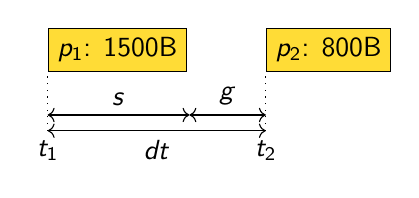
\begin{tikzpicture}
			[packet/.style={draw, fill=uofgsunshine}]
			\node[packet] (p1) {$p_1$: 1500B};
			\node[packet, right= 1cm of p1] (p2) {$p_2$: 800B};
			
			\node at ($(p1.south west) - (0,1)$) (t1) {$t_1$};
			\node at ($(p2.south west) - (0,1)$) (t2) {$t_2$};
			
			\draw[-, dotted] (t1.north)--(p1.south west);
			\draw[-, dotted] (t2.north)--(p2.south west);
			
			\draw[<->] (t1.north) -- node[below]{$dt$} (t2.north);
			\draw[<->] ($(t1.north) + (0,0.2)$) -- node[above]{$s$} ($(t1.north) + (1.8,0.2)$);
			\draw[<->] ($(t1.north) + (1.8,0.2)$) -- node[above]{$g$} ($(t2.north) + (0,0.2)$);
			\end{tikzpicture} 
		}
	\end{tikzfigure}
	Accurately measuring the ingress time of every packet allows us to approximate the time each packet spends on the wire.
	In turn, we can measure the \textbf{point rate} associated with each packet.
	Taken individually, these are counter-intuitive, but can reveal \textbf{interesting distributional characteristics} in aggregate (Fig. \ref{fig:bbr-cubic-rates}).
}
	\column{0.33}
	\block[bodywidthscale=0.9999]{Collectors---Stateful TCP Analysis}{
%	\begin{wrapfigure}[6]{r}{.3\linewidth}
		\fontsize{32}{38.4}\selectfont
		\vspace{-1em}
		\begin{tikzfigure}[Collector architecture.\label{fig:collector-arch}]
		\resizebox{\linewidth}{!}{\fontsize{10}{12}\selectfont\begin{tikzpicture}
		[stage/.style={draw, rounded rectangle, fill=brighterred, align=center, text=white},
		pipeline/.style={stage, fill=uofgrose},
		ws/.style={stage, fill=uofgslate, text=white},
		store/.style={stage, fill=uofgsunshine, text=black}]
		\node[draw, fill=white!90!uofgpumpkin, minimum width=10.5cm, minimum height=2.7cm] (collectorbox) at (4.6,0) {};
		\node[below right, inner sep=2pt] at (collectorbox.north west) {Collector};
		
		\node[stage](parse) {Parse};
		\node[stage, right = 0.4cm of parse](dispatch) {Dispatch};
		
		\node[pipeline, above right = 0.1cm and 0.7cm of dispatch](ana0) {Analyser 0};
		\node[pipeline, right = 0.3cm of ana0](serialiser0) {Serialiser 0};
		
		\node[pipeline, below right = 0.1cm and 0.7cm of dispatch](anan) {Analyser $n$};
		\node[pipeline, right = 0.3cm of anan](serialisern) {Serialiser $n$};
		
		\node at ($(ana0.south)!0.4!(anan.north)$) {$\vdots$};
		\node at ($(ana0.south)!0.4!(anan.north) + (0.2,-0.1)$) {$n$};
		\node at ($(serialiser0.south)!0.4!(serialisern.north)$) {$\vdots$};
		\node at ($(serialiser0.south)!0.4!(serialisern.north) + (0.2,-0.1)$) {$n$};
		
		\node[store, right = 7.4cm of parse](storage) {Shared\\Storage};
		
		\node[store, below = 1cm of storage] (tsdb) {Time-series\\Database};
		
		\node[ws, above right = 0.2cm and 2cm of storage](ws0) {WS Client 0};
		\node[ws, below right = 0.2cm and 2cm of storage](wsm) {WS Client $m$};
		\node at ($(ws0.south)!0.4!(wsm.north)$) {$\vdots$};
		\node at ($(ws0.south)!0.4!(wsm.north) + (0.25,-0.1)$) {$m$};
		
		\draw[thick, ->] (parse)--(dispatch);
		\draw[thick, ->] (dispatch)--(ana0.west);
		\draw[thick, ->] (dispatch)--(anan.west);
		
		\draw[thick, ->] (ana0)--(serialiser0);
		\draw[thick, ->] (anan)--(serialisern);
		
		\draw[thick, ->] (serialiser0)--(storage);
		\draw[thick, ->] (serialisern)--(storage);
		\draw[dashed, ->] (serialiser0)--(tsdb);
		\draw[dashed, ->] (serialisern)--(tsdb);
		
		\draw[<->] (storage)--(ws0.west);
		\draw[<->] (storage)--(wsm.west);
		
		\node[above = 1.3cm of parse] (locallabel) {Local};
		\node[right = 10.3cm of locallabel] (remotelabel) {Remote};
		
		\draw[-, dotted] ($(remotelabel) - (1,-0.5)$)--($(remotelabel) - (1,4.5)$);
		\end{tikzpicture}}
		\vspace{-2em}
		\end{tikzfigure}

		We implement a collector application in \textbf{Go} to perform TCP flow analysis from High Touch packets, including the following algorithms:
		\begin{itemize}
			\item Rate Monitoring (point estimate and sliding window).
			\item Packet loss and retransmission detection.
			\item Online SRTT via Karn's algorithm \cite{DBLP:journals/ccr/KarnP87}.
			\item Bytes-in-flight tracking.
			\item Congestion window size estimation via \citeauthor{DBLP:conf/sosr/GhasemiBR17}'s algorithm \cite{DBLP:conf/sosr/GhasemiBR17}.
		\end{itemize}
	
		We use a \textbf{pipelined design} (Fig. \ref{fig:collector-arch}) to maximise throughput where possible.
	\begin{tikztable}[Pipeline processing rates.\label{tab:rates}]
		\resizebox{\linewidth}{!}{\begin{tabular}{@{}ccccc@{}}
				\toprule\multicolumn{1}{c}{Metric} & \multicolumn{1}{c}{Parse} & \multicolumn{1}{c}{Dispatch} & \multicolumn{1}{c}{Analysis} & \multicolumn{1}{c}{Serialisation} \\ \midrule
				Packet rate (kpps) & 1300 & 775 & \numrange{310}{485} & 675 \\
				Flow rate, jumbo frames (\si{\giga\bit\per\second}) & 93.6 & 55.8 & \numrange{22.3}{34.9} & 48.6 \\
				Flow rate, \SI{1500}{\byte} (\si{\giga\bit\per\second}) & 15.6 & 9.3 & \numrange{3.7}{5.8} & 8.1 \\
				\bottomrule
			\end{tabular}
		}
	\end{tikztable}

	We instrument each stage using \textbf{Prometheus}; the ingress pipeline then has a peak capacity of \textbf{\SI{55.8}{\giga\bit\per\second} between all flows}, and \textbf{\SIrange{22.3}{34.9}{\giga\bit\per\second} per flow} (depending on which analyses are performed).
	Deployment machines will be considerably more powerful, and experiments in \emph{Rust} suggest higher parsing throughout.

%	\alert{Does this work?}
%	\end{wrapfigure}
}
	
\block[bodywidthscale=0.9999]{Measuring At Midpoints}{
	\fontsize{32}{38.4}\selectfont
	\begin{tikzfigure}[SRTT computation of unidirectional flows as seen by collectors. Packets carrying data are marked by a red arrow.\label{fig:srtt}]
		\resizebox{0.7\linewidth}{!}{\fontsize{8}{9.6}\selectfont
				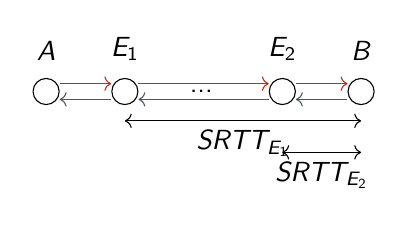
\begin{tikzpicture}[seq/.style={draw=brighterred}, ack/.style={draw=uofgslate}]
				\node[draw, circle] (acirc) {};
				\node[above = 0.1cm of acirc] {$A$};
				
				\node[draw, circle, right of = acirc] (e1circ) {};
				\node[above = 0.1cm of e1circ] {$E_1$};
				
				\node[right of = e1circ] (missingnet) {$\dots$};
				
				\node[draw, circle, right of = missingnet] (e2circ) {};
				\node[above = 0.1cm of e2circ] {$E_2$};
				
				\node[draw, circle, right of = e2circ] (bcirc) {};
				\node[above = 0.1cm of bcirc] {$B$};
				
				\draw[->, seq] ($(acirc.east) + (0.0,0.1)$) -- ($(e1circ.west) + (0.0,0.1)$);
				\draw[<-, ack] ($(acirc.east) - (0.0,0.1)$) -- ($(e1circ.west) - (0.0,0.1)$);
				
				\draw[->, seq] ($(e1circ.east) + (0.0,0.1)$) -- ($(e2circ.west) + (0.0,0.1)$);
				\draw[<-, ack] ($(e1circ.east) - (0.0,0.1)$) -- ($(e2circ.west) - (0.0,0.1)$);
				
				\draw[->, seq] ($(e2circ.east) + (0.0,0.1)$) -- ($(bcirc.west) + (0.0,0.1)$);
				\draw[<-, ack] ($(e2circ.east) - (0.0,0.1)$) -- ($(bcirc.west) - (0.0,0.1)$);
				
				\draw[<->] ($(e1circ.south) - (0.0,0.2)$) -- node[below]{$SRTT_{E_1}$} ($(bcirc.south) - (0.0,0.2)$);
				\draw[<->] ($(e2circ.south) - (0.0,0.6)$) -- node[below]{$SRTT_{E_2}$} ($(bcirc.south) - (0.0,0.6)$);
				
				\end{tikzpicture}
			}
		\vspace{-1em}
	\end{tikzfigure}

%	?? Discuss how we can diagnose our own network and part of the recipient, process of elimination
	Given that many flows are effectively unidirectional in byte volume, TCP analysis performed between endpoints means that \textbf{certain metrics describe a portion of the path} (SRTT, bytes in flight).
	Gathering these metrics at \textbf{both WAN ingress/egress} may be useful for diagnosing anomalous path behaviour.
}
	\block[bodywidthscale=0.9999]{TCP Flavour Rate Distribution}{
		\fontsize{32}{38.4}\selectfont
		\begin{tikzfigure}[Point (blue) and sliding window (red) rates at \SI{1}{\giga\bit\per\second}. TCP Cubic is on the left, BBR is on the right.\label{fig:bbr-cubic-rates}]
		\resizebox{0.49\linewidth}{!}{
			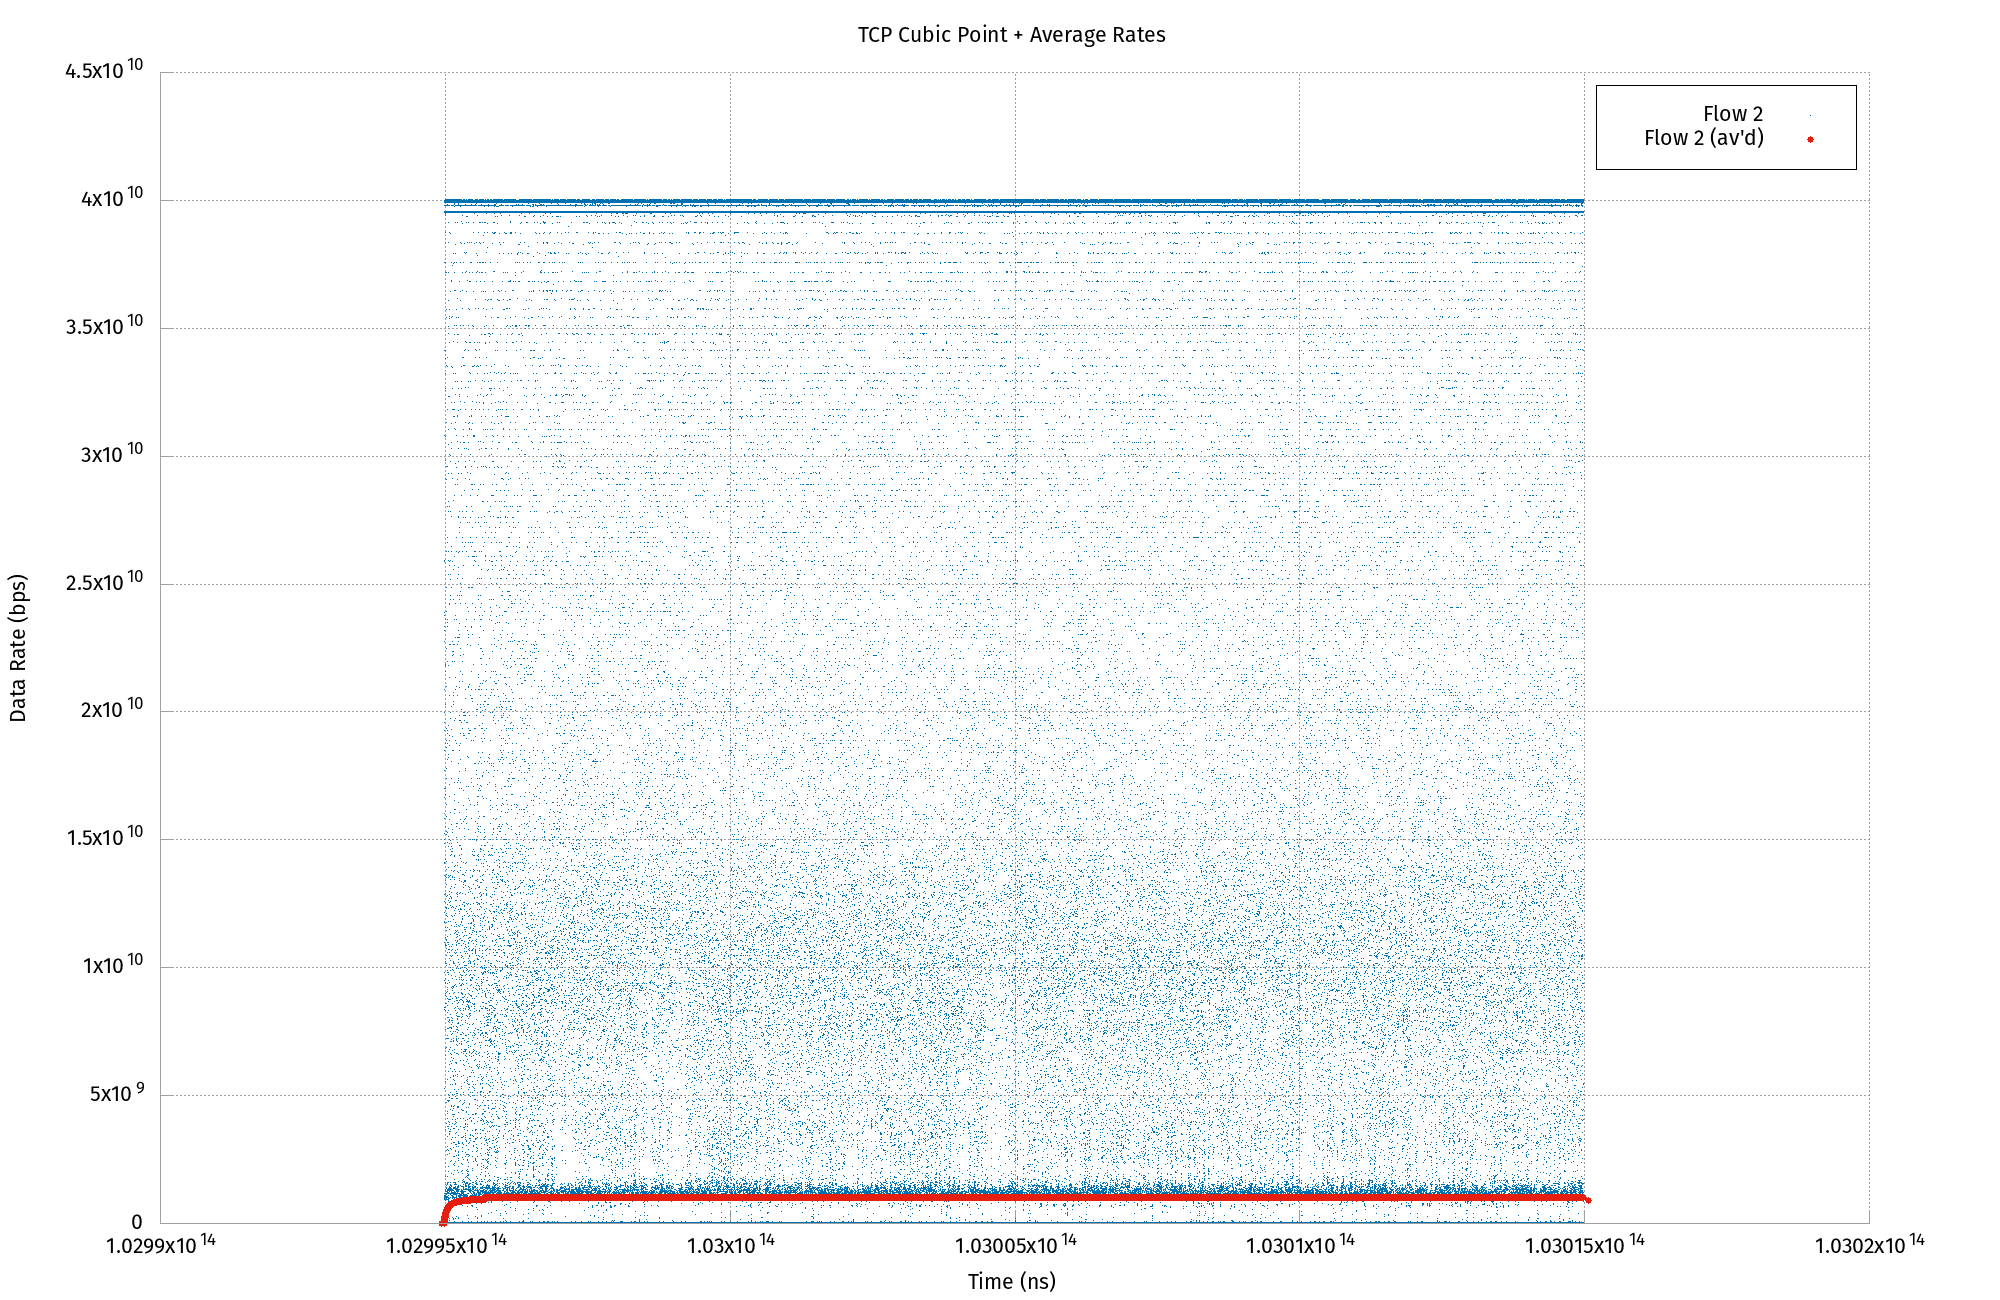
\includegraphics{cubic-point-rates}
		}
		\resizebox{0.49\linewidth}{!}{
			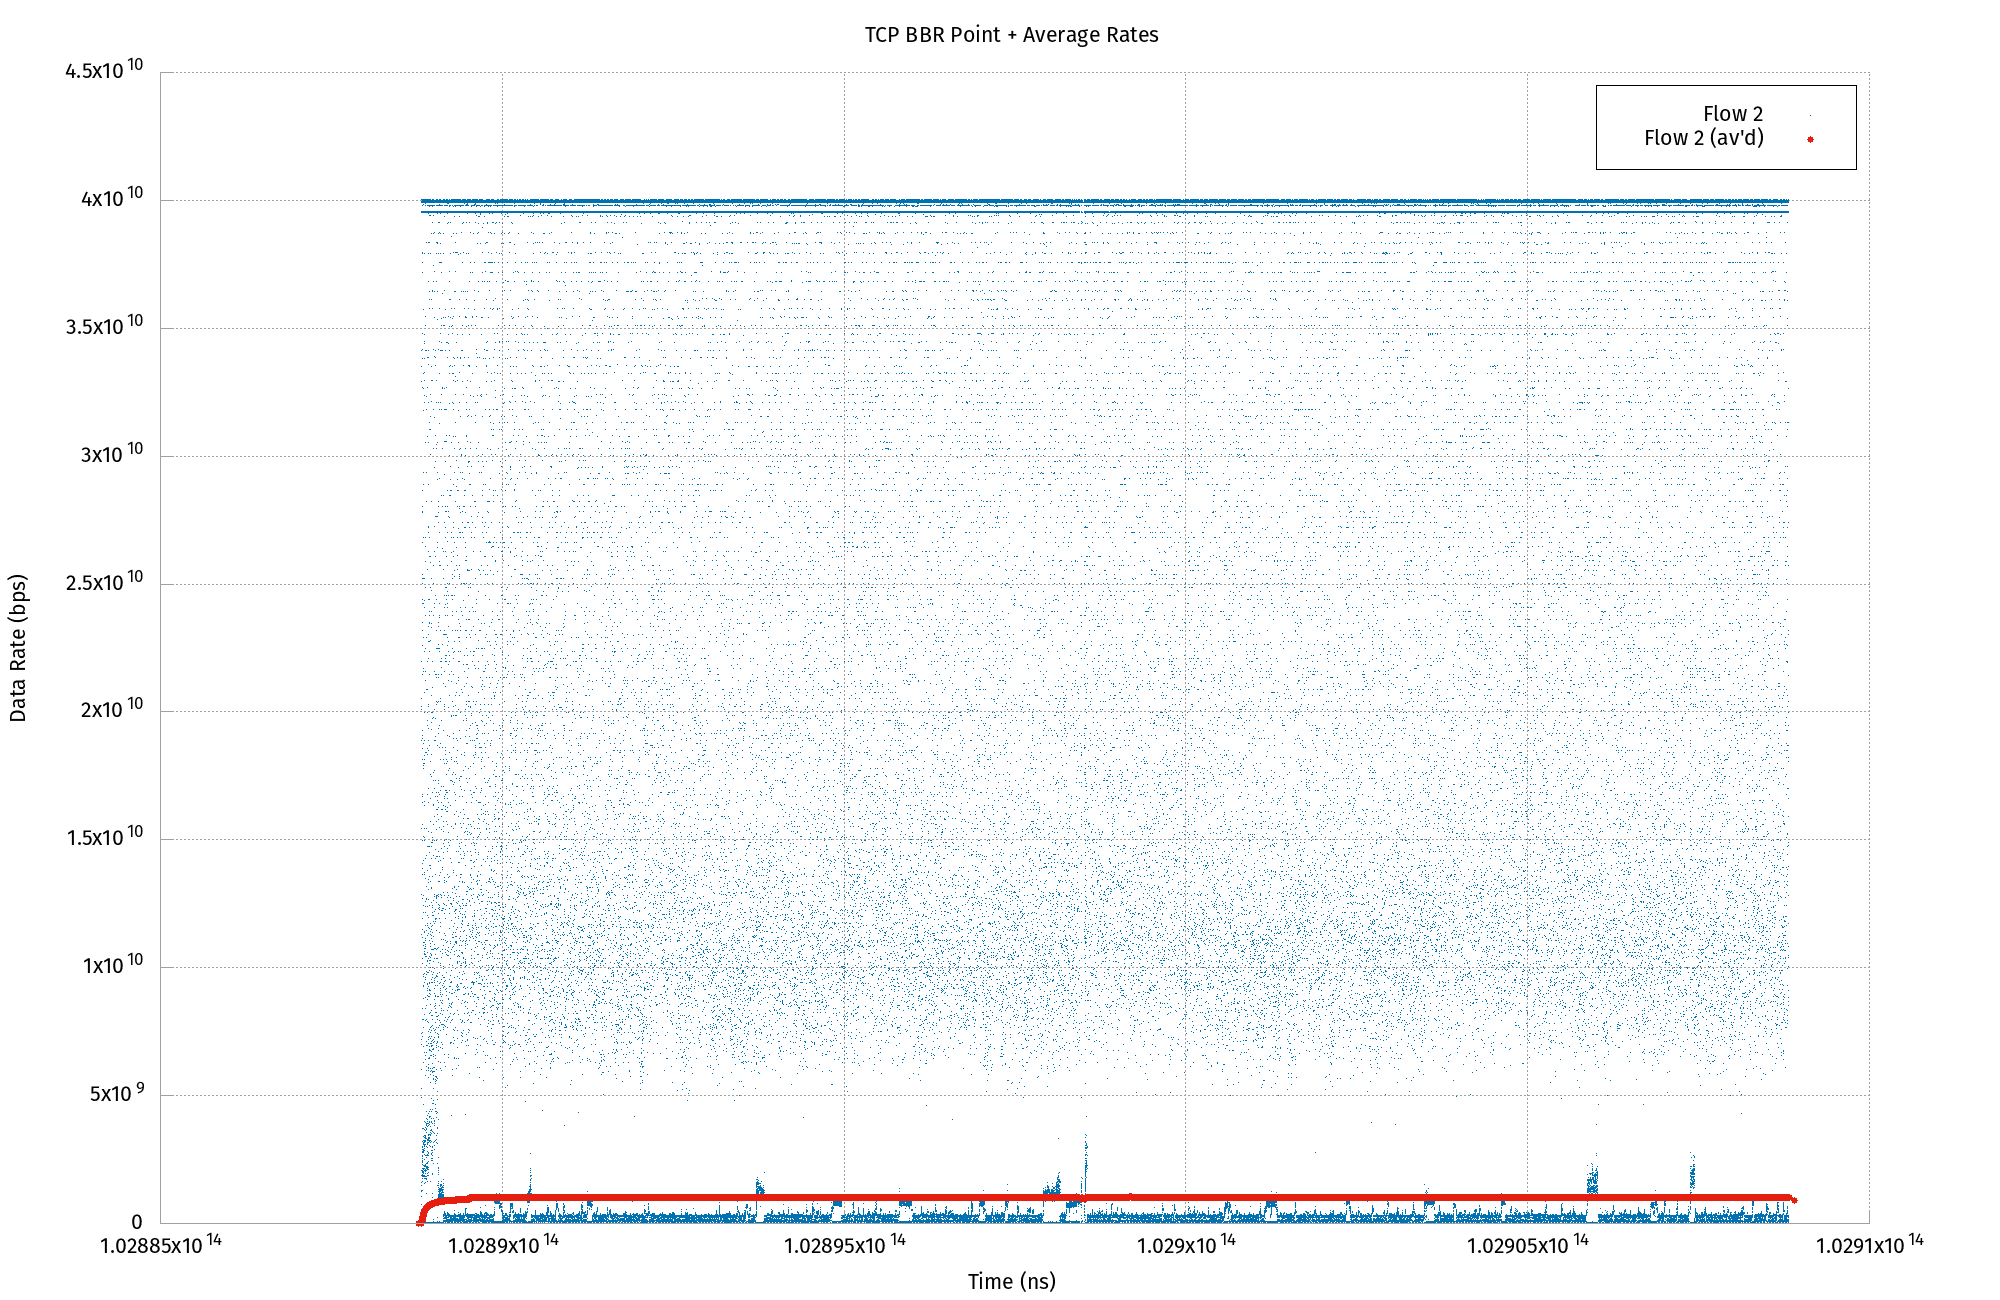
\includegraphics{bbr-point-rates}
		}
		\end{tikzfigure}
		Distributions of point rates over time vary for different flows---\textbf{suggesting e.g., different congestion control algorithm behaviour}.
		Close inspection reveals that \textbf{BBR point rates have more structured distribution}.
	}
	\column{0.33}
	\block[bodywidthscale=0.9999]{Next Collectors}{
		\fontsize{32}{38.4}\selectfont
		Stateful TCP analysis of this kind acts as a \textbf{pilot project} for the feasibility of the system. We intend to explore other collector designs, including:
		\begin{itemize}
			\item \textbf{Peak utilisation tracking} (i.e., at \SI{1}{\second} granularity).
			\item \textbf{Monitoring microbursts} in the network via timing information.
			\item Visualisation/measurement of \textbf{queueing}.
		\end{itemize}
	}
	\block[bodywidthscale=0.9999]{TCP Flavour Identification}{
		\begin{tikzfigure}[Accuracy in telling apart TCP Cubic and BBR flows.\label{fig:lstm}]
			\adjincludegraphics[width=0.94\linewidth]{cubic-vs-bbr-accuracy-poster}
		\end{tikzfigure}
	Motivated by the differences in point rate distribution between flows, we have have begun preliminary testing of TCP flavour identification using \textbf{long short-term memory} (LSTM) networks \cite{DBLP:journals/neco/HochreiterS97}, which are well suited to time-series classification.
	We currently see \textbf{\SI{98.9}{\percent} prediction accuracy in as few as 20 measurements} for unmultiplexed flows.
	}
	\block[bodywidthscale=0.9999]{Datasets}{
		\fontsize{32}{38.4}\selectfont
		We provide telemetry packet captures and collector output for solo and pairs of multiplexed flows for $\left\{100,200,\ldots,1000\right\}$\si{\mega\bit\per\second}, using TCP \emph{Cubic}, \emph{BBR}, \emph{Reno} and \emph{Vegas} in \emph{iperf3}.
		This is available at: \\ \textbf{\url{https://tinyurl.com/esnet-ht-data}}.
	}
	\block[bodywidthscale=0.9999]{Future Work}{
		\fontsize{32}{38.4}\selectfont
		\begin{itemize}
			\item \textbf{Correlating results between collectors} (and switch-to-switch time synchronisation \cite{DBLP:conf/sosr/KannanJC19}).
			\item Move control of \textbf{which analyses are performed} to the control plane.
			\item Investigate \textbf{analysis \emph{on} SmartNICs}.
			\item Handling \textbf{asymmetric flows}.
		\end{itemize}
	}
	\block{References}{\renewcommand*{\bibfont}{\footnotesize}\selectfont\printbibliography[heading=none]}
\end{columns}
\end{document}
%\maketitle